\documentclass{report}
\usepackage[utf8]{inputenc}
\usepackage{kotex}
\usepackage{xeCJK}
\usepackage{CJKutf8}
\usepackage[pdftex]{graphicx}

\title{OpenSourceSW TeamProject-05}
\author{이행석 송남주 하지민}
 
\begin{document}

    \maketitle
    \begin{flushleft}  
    
    
    
    \tableofcontents{}

    \Large
    \chapter{오픈 소스 SW  개요 및 설치}
     \section{본 오픈소스 선택 이유}
      \begin{itemize}
        \item 현재 많은 오픈 소스 소프트웨어 툴들이 존재하지만, 대부분은 작업을 수행함에 있어 편리함을 추구하기 위하여 배포되고 있습니다.
        \item 이에 따라 본 팀은 흥미를 위한 게임 분야에도 오픈 SW가 있는 가에 대한 의문을 품게 되었으며, 여러 조사를 통해 Hedgewars라는 게임을 선택하게 되었습니다.
    \end{itemize}
     \section{오픈 소스 SW 개요}
      \begin{itemize}
        \item 턴 제 전략 게임인 Worms와 유사합니다
        \item 플레이어 마다 각 턴이 주어지며, 해당 턴의 시간 안에 마음껏 위치를 변경하여 여러 무기들 중 하나를 골라 상대방에게 피해를 입히는 게임입니다.
        \item 싱글플레이와 멀티플레이를 지원하며, 게임에 어려움을 느낄 사람들을 위해 트레이닝 맵도 마련되어 있습니다.
        \item 언어 또한 해당 OS의 설정 언어에 맞추어 변경 되므로, 언어 사항에 제약이 따르지 않습니다.
        \item  Windows 와 모바일 iOS 환경에서 제공이 되며 설치를 통해 실행 가능합니다.
    \end{itemize}
    \begin{figure}[h!]
\centering
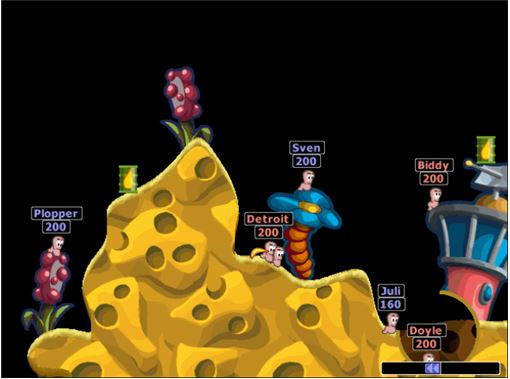
\includegraphics[scale=0.8]
{Image/worms.JPG}
\caption{실제 worms 플레이 화면}
\label{fig:detect}
\end{figure}

    \begin{figure}[h!]
\centering
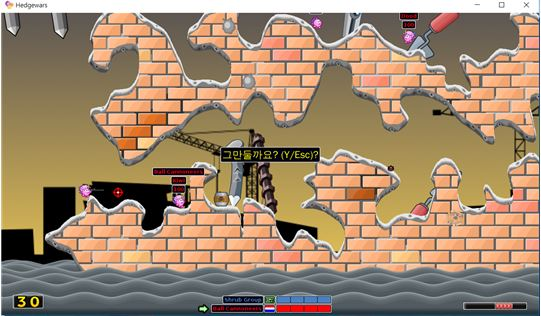
\includegraphics[scale=0.8]
{Image/HedgeWars.JPG}
\caption{실제 Hedgewars 플레이 화면}
\label{fig:detect}
\end{figure}
  \section{설치 방법}
  \subsection{홈페이지 접속}
    \begin{itemize}
  \item http://www.hedgewars.org/ 사이트를 통해 Hedgewars를 다운로드 받을 수 있습니다.
  \item 현재 나와 있는 릴리즈 버전과 배포 일자, 변경점 및 다운로드 링크와 오른쪽에는 멀티플레이를 할 때 필요한 계정 생성, 현재 서버 내에 개설된 방과 플레이 중인 인원 수가 나와 있습니다.
   \end{itemize}
   \begin{figure}[h!]
\centering
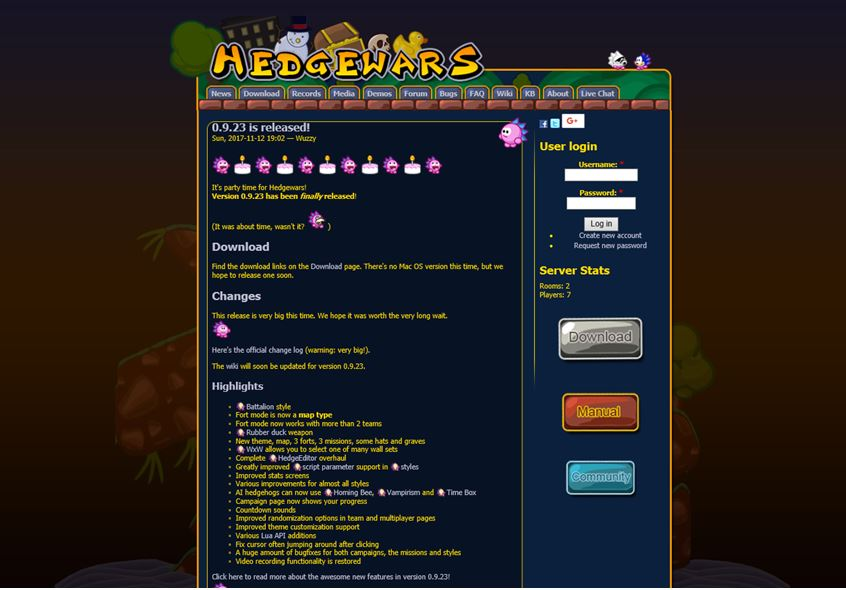
\includegraphics[scale=0.8]
{Image/homepage.JPG}
\caption{Hedgewars 사이트의 모습}
\label{fig:detect}
\end{figure}
  \subsection{다운로드 링크}
   \begin{itemize}
  \item 상단 혹은 우측의 Download 버튼을 통해 이동합니다.
  \item 윈도우 버전 내의 인스톨 파일과 토렌트 파일이 존재하며, 소스 코드 또한 제공해 주고 있습니다. 최신 릴리스 버전 하단에는 패키지 매니저를 제공하며, 그 밑에는 iOS 다운로드 링크와 git의 repository를 보여주고 있습니다.
  \item 그림에 표시된 다운로드 링크를 통해 설치를 진행합니다.
     \end{itemize}
      \begin{figure}[h!]
\centering
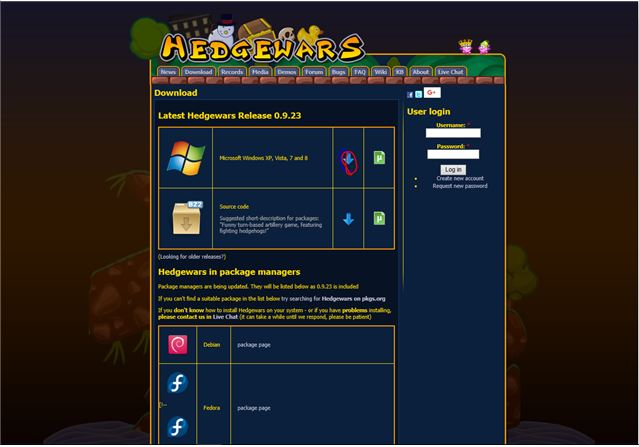
\includegraphics[scale=0.8]
{Image/download.JPG}
\caption{다운로드 링크 진입 시 화면}
\label{fig:detect}
\end{figure}
  \subsection{라이센스 동의}
    \begin{itemize}
  \item 실행 창이 시작되면 다음을 눌러준 후 라이센스에 관한 사항을 읽고 동의함을 클릭합니다.
     \end{itemize}
      \begin{figure}[h!]
\centering
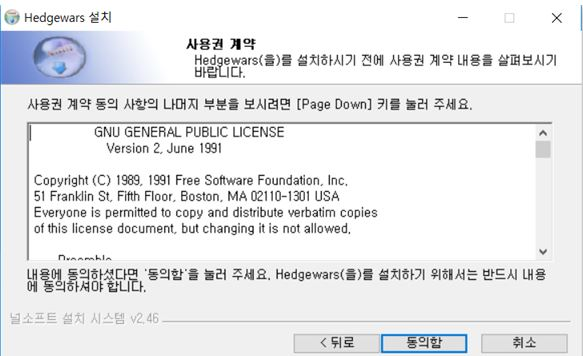
\includegraphics[scale=0.8]
{Image/install2.JPG}
\caption{라이센스 동의 확인 창}
\label{fig:detect}
\end{figure}
    \chapter{게임 메뉴 및 옵션}
     \section{메인 메뉴}
     \begin{itemize}
        \item 왼쪽은 싱글플레이, 오른쪽은 네트워크플레이를 나타냅니다.
        \item 싱글 플레이시 하나의 컴퓨터로 게임을 하고 친구나 AI가 제어하는 팀과 겨루게 됩니다.
        \item 네트워크 플레이시 친구와 전용서버를 이용해 플레이 하거나, 공식서버에서 플레이 할 수 있습니다.
    \end{itemize}
        \begin{figure}[h!]
\centering
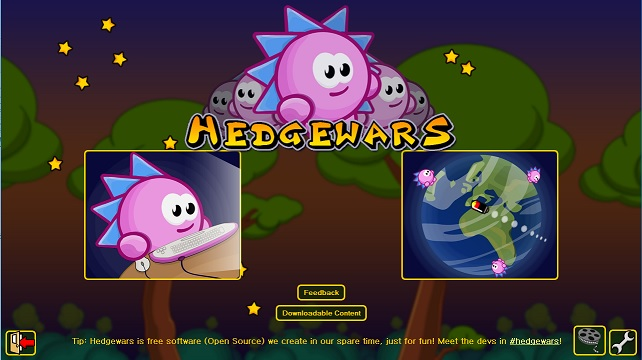
\includegraphics[scale=0.8]
{Image/main.jpg}
\caption{게임 실행시 초기 화면}
\label{fig:detect}
\end{figure}
     \section{싱글플레이}
    \begin{itemize} 
        \item 싱글플레이를 들어가면 나오는 메뉴는 총 4가지가 존재합니다.
        \item 빠른 대전
        \\ AI 혹은 친구와 멀티플레이 모드
        \\ 캠페인모드
        \\ 트레이닝모드
    \end{itemize}
            \begin{figure}[h!]
\centering
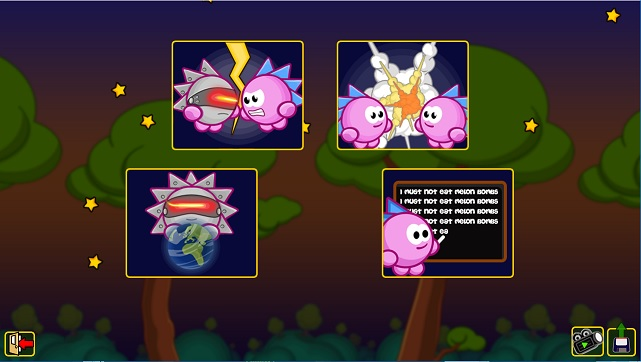
\includegraphics[scale=0.8]
{Image/single.jpg}
\caption{싱글플레이 선택 후 나오는 메뉴}
\label{fig:detect}
\end{figure}
     \subsection{빠른 대전}
     \begin{itemize}
         \item 매 판마다 새로운 설정으로 컴퓨터와 게임을 하게 됩니다.
         \item 사용자가 원하는 설정으로 플레이 할 수는 없습니다.
     \end{itemize}
     \subsection{멀티플레이 모드}
     \begin{itemize}
         \item 사용자가 원하는 맵과 게임설정을 선택하고 AI 혹은 친구와 대전을 하는 게임모드입니다.
         \item Random 버튼을 누르면 모든 설정을 임의적으로 할 수 있습니다.
         \item 조종하는 캐릭터는 최소 1에서 최대 8까지 가능하고 친구 한명과 AI 3명까지 설정 가능합니다.
     \end{itemize}
          \begin{figure}[h!]
\centering
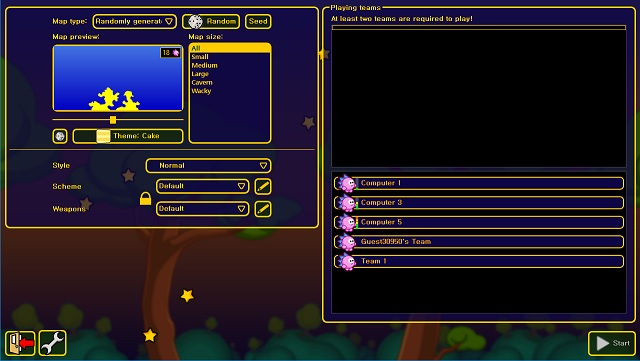
\includegraphics[scale=0.8]
{Image/Smulti.jpg}
\caption{멀티플레이 모드 화면}
\label{fig:detect}
\end{figure}
     \subsection{캠페인 모드}
     \begin{figure}[h!]
\centering
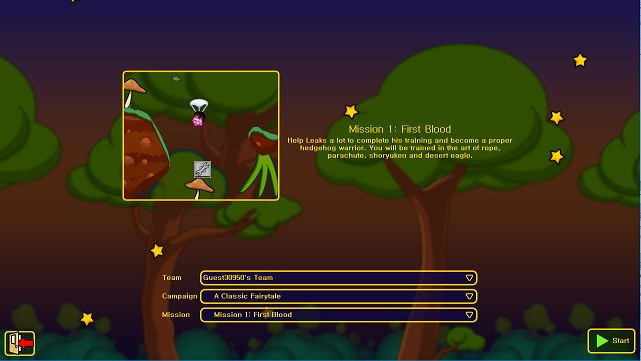
\includegraphics[scale=0.8]
{Image/Scampaign.jpg}
\caption{캠페인 모드 화면}
\label{fig:detect}
\end{figure}
     \begin{itemize}
         \item 사용자가 스토리에 따른 미션을 진행하는 모드로 ‘클래식 동화’ 캠페인과 ‘우주 어드벤처’ 캠페인 총 2가지가 존재합니다.
         \item 각 캠페인 미션에는 주요미션과 사이드 미션으로 여러 개의 미션들이 존재하며 각 미션들을 클리어 하면서 스토리를 진행하는 방식입니다
     \end{itemize}
     \subsection{싱글 미션}
     \begin{itemize}
         \item  싱글 미션에는 총 3가지 모드가 있습니다.
         \item training missions, challenges, scenarios 가 존재하며	게임을 진행하는데 있어 필요한 기술들을 교육시켜주는 모드입니다. 
     \end{itemize}
     
     \begin{figure}[h!]
\centering
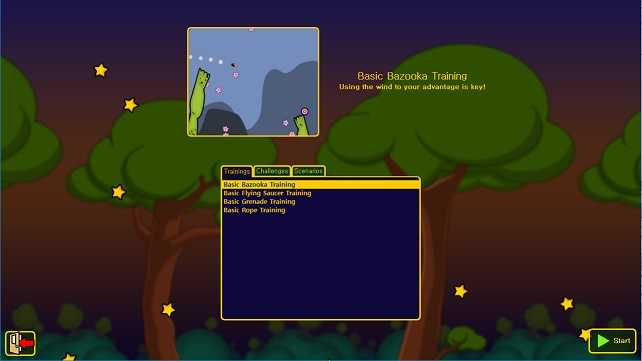
\includegraphics[scale=0.8]
{Image/Straining.jpg}
\caption{싱글 미션 화면}
\label{fig:detect}
\end{figure}
     
     
     \section{네트워크 플레이}
     \begin{figure}[h!]
\centering
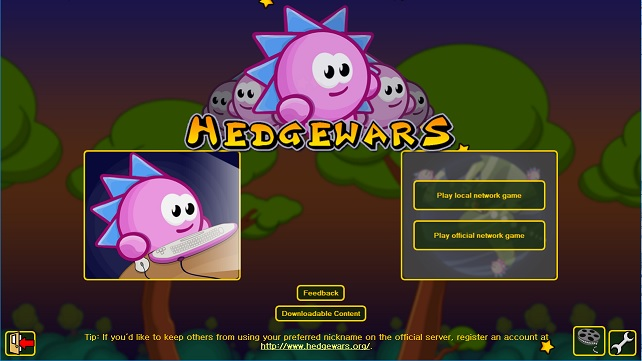
\includegraphics[scale=0.8]
{Image/network.jpg}
\caption{네트워크 플레이 선택 화면}
\label{fig:detect}
\end{figure}
     
     \begin{itemize}
         \item 네트워크 플레이를 선택하면 2가지 메뉴가 나타납니다.
         \\local network game
         \\official network game
     \end{itemize}
     
     \subsection{local network game}
     \begin{itemize}
         \item  LAN을 이용해 자신과 같은 네트워크에 있는 사람과 게임을 하고싶을 때 사용 할 수 있는 네트워크 플레이입니다.
         \item  start server 버튼으로 새로운 LAN서버 게임을 만들 수 있고 서버이름과 포트를 입력하면 생성이 완료됩니다.
     \end{itemize}
     
     \begin{figure}[h!]
\centering
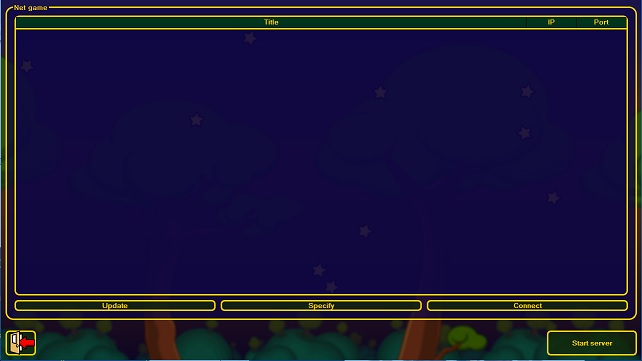
\includegraphics[scale=0.8]
{Image/localnet.jpg}
\caption{로컬 네트워크 게임}
\label{fig:detect}
\end{figure}
     
     
     \subsection{official network game}
     
     \begin{itemize}
         \item hedgewars에서 제공하는 공식서버에서 전 세계 사람들과 할수 있는 네트워크 플레이입니다.
         \item 게임을 찾는 동안 채팅박스에서 자유롭게 채팅을 할수도 있습니다. 원하는 게임이 있으면 그 방으로 접속해 게임을 즐기거나, Create room 버튼으로 새로운 방을 만들 수 있습니다.
     \end{itemize}
     
     \begin{figure}[h!]
\centering
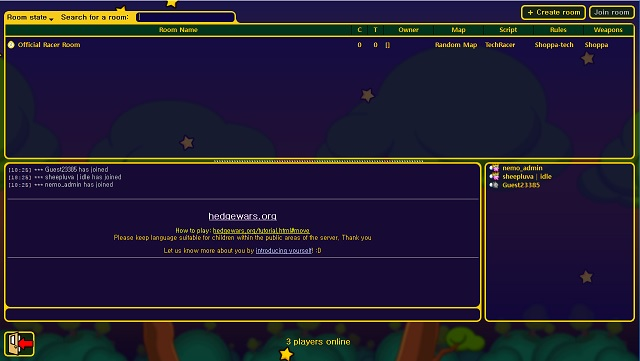
\includegraphics[scale=0.8]
{Image/officialnet.jpg}
\caption{오피셜 네트워크 게임}
\label{fig:detect}
\end{figure}


\section{옵션 상의 각 Scheme, Weapon 모드}
\subsection{Scheme 모드}
\begin{itemize}
    \item Scheme는 Hedgewars에서 많은 게임 모드를 설정하는 데 사용됩니다. 
    \item Pro mode : 15초 이동과 제한된 무기, 스킬만 사용가능합니다.
    \item Shoppa mode : 30초 이동이 가능하며, Shopping을 할 수 있습니다.
\end{itemize}
\subsection{Weapon 모드}
\begin{itemize}
    \item 무기의 종류를 선택선택할 수 있습니다.
\end{itemize}

   \begin{figure}[h!]
\centering
\includegraphics[scale=0.8]
{Image/Scheme.JPG}
\caption{옵션 상의 각 Scheme, Weapon 모드}
\label{fig:detect}
\end{figure}



     
     
    \chapter{키 설명 및 게임 방법}
     \section{초기 게임 화면}
    \begin{figure}[h!]
    \centering
    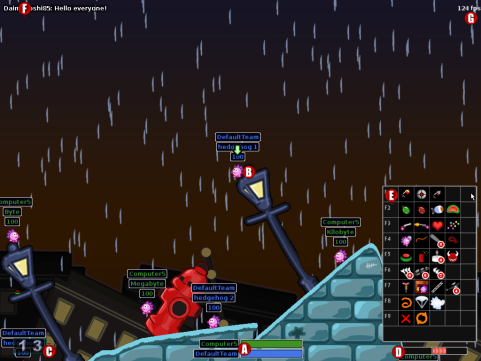
\includegraphics[scale=0.8]
    {Image/Gamescreen.png}
    \caption{초기 게임 화면}
    \label{fig:detect}
    \end{figure}
     \large
    \subsection{팀 체력바}
    \begin{itemize}
        \item 각 팀의 총 체력을 나타냅니다.
        \item 고슴도치(플레이어가 조종하는 캐릭터, 2번)들이 공격당하면, 해당 고슴도치가 속한 팀의 체력 바가 감소합니다.
    \end{itemize}
    \subsection{고슴도치}
    \begin{itemize}
        \item 플레이어와 컴퓨터가 움직이는 캐릭터입니다. 
        \item 무기를 들고 상대 고슴도치를 공격해서 상대방의 모든 고슴도치를 잡는 것이 주 목표입니다.
    \end{itemize}
    \subsection{제한시간}
        \begin{itemize}
        \item 고슴도치가 움직이거나 공격할 수 있는 제한 시간입니다. 
        \item 제한 시간이 지나면 상대팀에게 턴이 넘어갑니다.
    \end{itemize}
    \subsection{바람세기}
    \begin{itemize}
        \item 바람이 어느 방향으로 얼마나 세게 부는 지를 나타냅니다.
        \item 바의 가리키는 방향 표시가 길면 길수록 세기가 강합니다.
    \end{itemize}
    \subsection{무기메뉴}
    \begin{itemize}
        \item 이번 게임에서 플레이어가 사용할 수 있는 무기를 테이블 형태로 나열해 놓았습니다. 
        \item 무기 메뉴 중 하나를 선택하면 플레이어가 움직이는 고슴도치가 선택한 무기를 지닙니다.
        \item 빨간색 원 표시가 있는 회색 무기들은 빨간색 원에 안에 있는 숫자 턴만큼만 해당 무기를 사용할 수 있습니다. 
    \end{itemize}
    \subsection{채팅}
    \begin{itemize}
        \item 멀티플레이 시 플레이어와 상대방의 가장 최근 대화 내용을 볼 수 있습니다. 
    \end{itemize}
    \subsection{FPS}
    \begin{itemize}
        \item 게임 진행 간 초당 프레임 수를 나타냅니다. 
    \end{itemize}
    
    \section{기본적인 움직임 및 슈팅}
    \begin{figure}[h!]
    \centering
    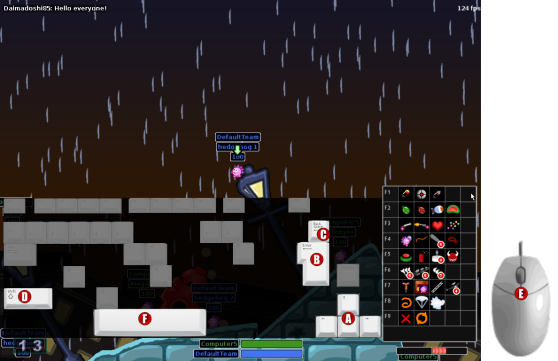
\includegraphics[scale=0.8]
    {Image/Basicmoveshot.png}
    \caption{기본적인 움직임 및 슈팅}
    \label{fig:detect}
    \end{figure}
    \subsection{Cursor keys}
    \begin{itemize}
        \item ← → 키를 이용해 고슴도치를 왼쪽 또는 오른쪽으로 움직일 수 있습니다.
        \item ↑ ↓ 키를 이용해 무기 조준점을 움직일 수 있습니다.
    \end{itemize}
    \subsection{Enter}
    \begin{itemize}
        \item 현재 선택된 고슴도치가 앞으로 점프합니다. 
        \item 너무 높은 곳에서 떨어지면 체력 바가 닳게 됩니다.
        \item 로프나 비행접시를 사용해 이동하는 동안, 엔터를 활용해서 무기를 던지거나 떨어트릴 수 있습니다. 예를 들어, 로프를 사용하면서 다이너마이트를 떨어트릴 수 있습니다.
    \end{itemize}
    \subsection{Backspace}
    \begin{itemize}
        \item 한 번 누르면 수직으로 점프하고
 두 번 누르면 뒤로 점프합니다. 
        \item 백스페이스를 두 번째 누를 때 좀 더 긴 시간을 두고 누르면 더 높게 점프합니다.
    \end{itemize}
    \subsection{Left Shift}
    \begin{itemize}
        \item 표적을 정확히 조준할 때 사용합니다. 
        \item 시프트를 누른 채 조준 키를 움직여 천천히 조준점을 이동하여 정밀 사격이 가능합니다.
        \item  이 키를 누른 상태에서 왼쪽이나 오른쪽으로 움직여도 움직이지 않고 제자리에서 방향 전환만 합니다.
    \end{itemize}
    \subsection{Mouse Clicks}
    \begin{itemize}
        \item 마우스 오른쪽을 클릭하면 무기 메뉴를 보여줍니다.
        \item 마우스 왼쪽을 클릭하면 메뉴에서 무기를 선택하거나, 공습과 같은 공격 타겟을 설정할 수 있습니다.
    \end{itemize}
    \subsection{Space bar}
    \begin{itemize}
        \item 플레이어의 고슴도치가 선택한 무기를 가지고 조준하고 있는 방향으로 공격할 수 하도록 만듭니다.
        \item 길게 누를수록 무기를 발사하는 힘이 강해집니다.
    \end{itemize}
    
    \section{조준 및 무기 변경}
    \begin{figure}[h!]
    \centering
    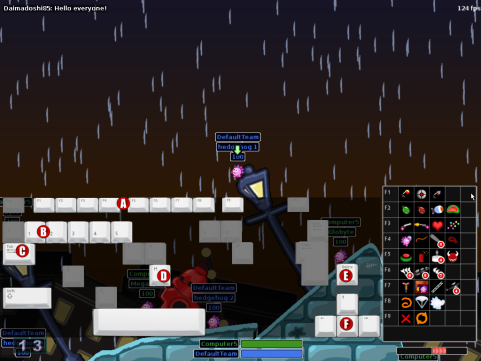
\includegraphics[scale=0.8]
    {Image/weaponmodifier.png}
    \caption{조준 및 무기 변경}
    \label{fig:detect}
    \end{figure}
    \subsection{F1 TO F10}
    \begin{itemize}
        \item 마우스 오른쪽 버튼을 클릭하는 대신 F1-F10을 사용해 무기를 변경할 수 있습니다.
    \end{itemize}
    \subsection{1 TO 5}
    \begin{itemize}
        \item 수류탄과 같은 일정 시간 후 폭발하는 무기의 시간을 설정할 수 있습니다. 
    \end{itemize}
    \subsection{TAB}
    \begin{itemize}
        \item 플레이어가 가지고 있는 고슴도치 내에서 움직이고자하는 고슴도치를 전환합니다. 
    \end{itemize}
    \subsection{H}
    \begin{itemize}
        \item 현재 선택된 고슴도치가 카메라 중앙으로 오도록 합니다.
    \end{itemize}
    \subsection{Delete}
    \begin{itemize}
        \item 팀 체력바가 화면에 보이지 않도록 만듭니다. 
    \end{itemize}
    
    
    \section{게임 옵션과 채팅 커맨드}
    \begin{figure}[h!]
    \centering
    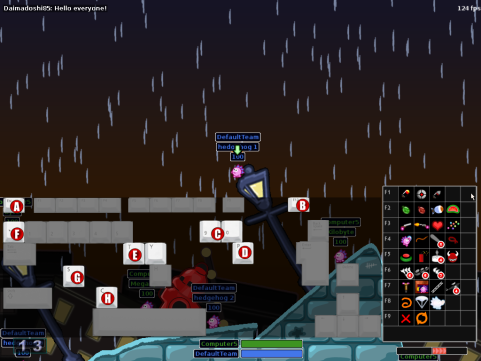
\includegraphics[scale=0.8]
    {Image/option.png}
    \caption{게임 옵션과 채팅 커맨드}
    \label{fig:detect}
    \end{figure}
    \subsection{ESC}
    \begin{itemize}
        \item 게임에서 나갑니다. 
        \item 임무 패널을 표시합니다. 
    \end{itemize}
    \subsection{F12}
    \begin{itemize}
        \item 전체화면 혹은 창화면으로 변경합니다. 
    \end{itemize}
    \subsection{9 AND 0}
    \begin{itemize}
        \item 게임 사운드 볼륨을 낮추거나 키웁니다.
    \end{itemize}
    \subsection{P}
    \begin{itemize}
        \item 오프라인 모드에서 게임을 일시 중지 시킵니다.
        \item 라인 모드에서는 AFK모드로 전환합니다.
        \item 임무 패널을 표시합니다.
    \end{itemize}
    \subsection{T}
    \begin{itemize}
        \item 채팅 메시지를 보냅니다. 
    \end{itemize}
    \subsection{`}
    \begin{itemize}
        \item 과거 채팅 기록을 보여줍니다. 
    \end{itemize}
    \subsection{C}
    \begin{itemize}
        \item 스크린샷을 찍고 저장합니다. 
    \end{itemize}
    
    \section{추가 제어키}
    \subsection{Y}
    \begin{itemize}
        \item 같은 팀끼리만 보이는 채팅을 합니다. 
    \end{itemize}
    \subsection{Left Shift}
    \begin{itemize}
        \item 얼음이 많은 지형에서 미끄러지는 것을 방지하십시오. 
    \end{itemize}
    \subsection{Left Shift + Tab}
    \begin{itemize}
        \item 고슴도치를 역순으로 전환한다.
    \end{itemize}
    \subsection{Left Shift + Delete}
    \begin{itemize}
        \item HUD 숨김
    \end{itemize}
    \subsection{Left Shift + Tab + Delete}
    \begin{itemize}
        \item 전체 현재 지도의 이미지와 마스크를 만들어 사용자 디렉토리의 스크린 샷 폴더에 저장합니다.
    \end{itemize}
    
    
    
     \chapter{발견된 버그 및 기능 향상 제안}
     \section{발견된 버그}
     \begin{itemize}
        \item 고무줄이 예상치 못한 곳에서 나타나거나 사라지는 현상이 발생합니다.
          \begin{figure}[h!]
\centering
\includegraphics[scale=0.8]
{Image/Rubberband.JPG}
\caption{고무줄이 나타나거나 사라지는 현상}
\label{fig:detect}
\end{figure}
        \item 바다 맵에서 가장자리로 이동시 CRASH 발생합니다.
        \item 트레이닝 모드시 몇몇 목표물(타겟)이 파괴되지 않을 때 가 있습니다.
    \end{itemize}
     \section{기타 기능 향상을 위한 제안점}
     \begin{itemize}
         \item 한글화가 보다 잘 되어 있으면 좋겠습니다.
            \\ 중간중간 문맥에 맞지 않는 어구나 영어가 있어 친숙하지 않는 사람에겐 사용하기 어려울 수 있습니다.
        \item 좀 더 빠른 버그 대응책이 필요합니다.
            \\ 게임 내 버그 발생시 알릴 수 있는 페이지가 있지만 실제로 반영되는데 너무 긴 시간이 걸립니다.
     \end{itemize}
    
    
      \chapter{협업 자료 첨부}
     \section{Repository}
       \begin{figure}[h!]
\centering
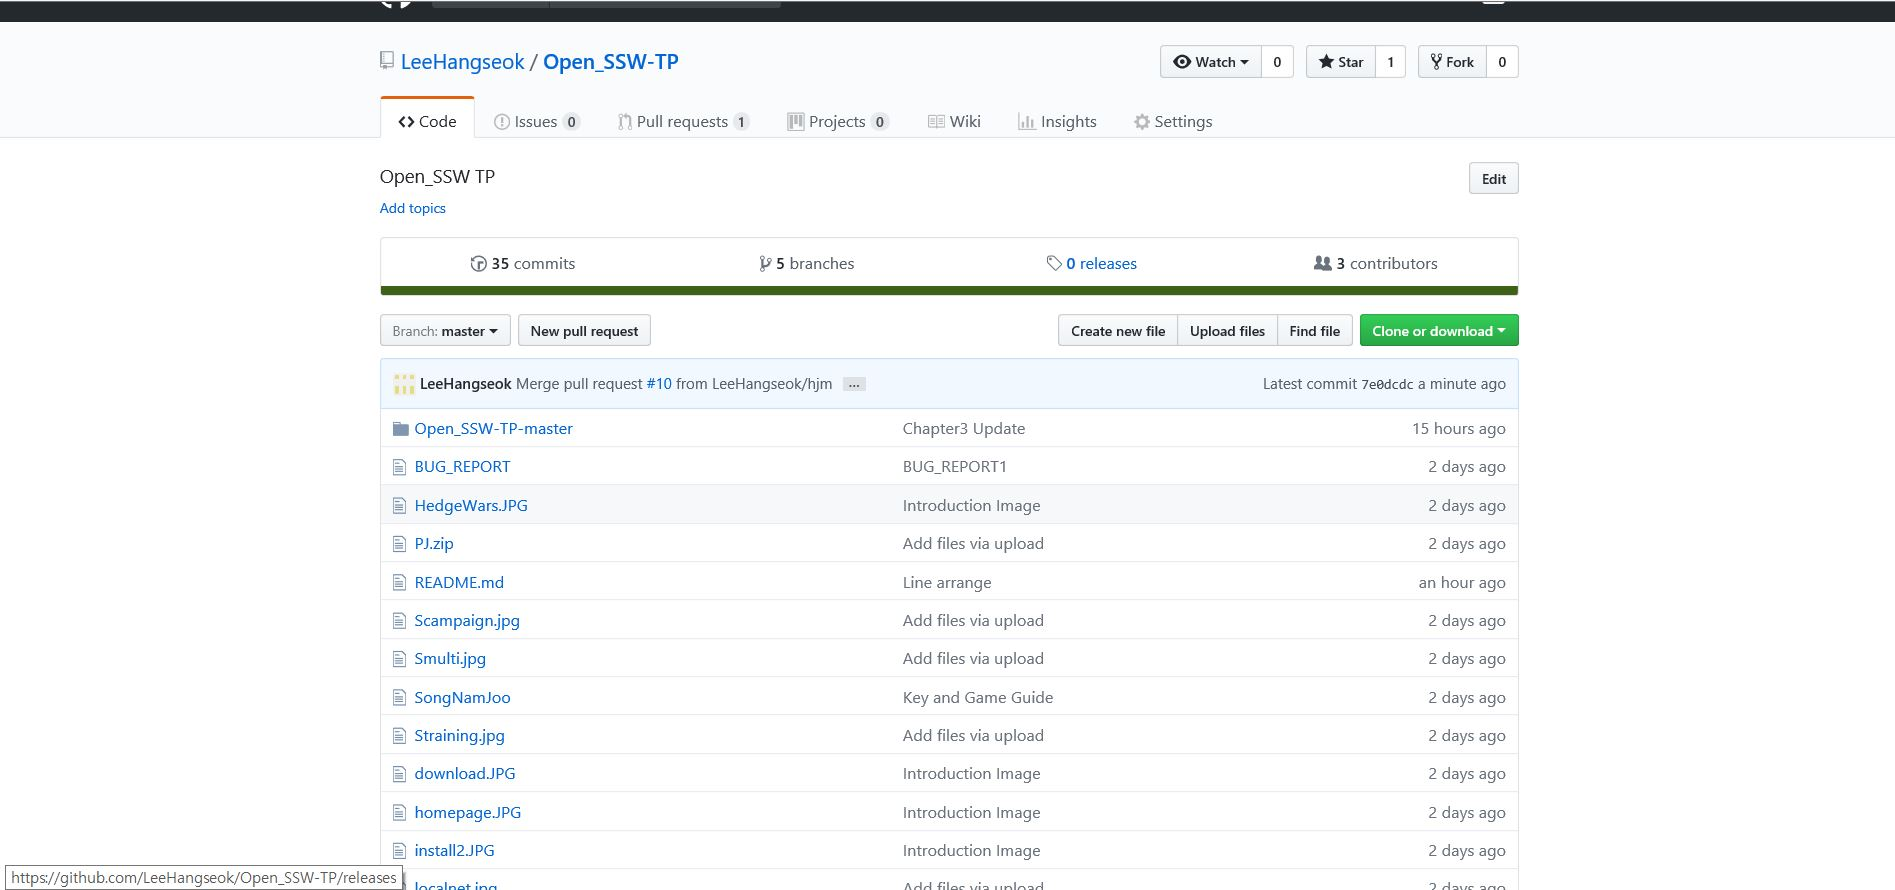
\includegraphics[scale=0.6]
{Image/Repository.JPG}
\caption{Repository 캡쳐본}
\label{fig:detect}
\end{figure}
     \section{Pulse}
       \begin{figure}[h!]
\centering
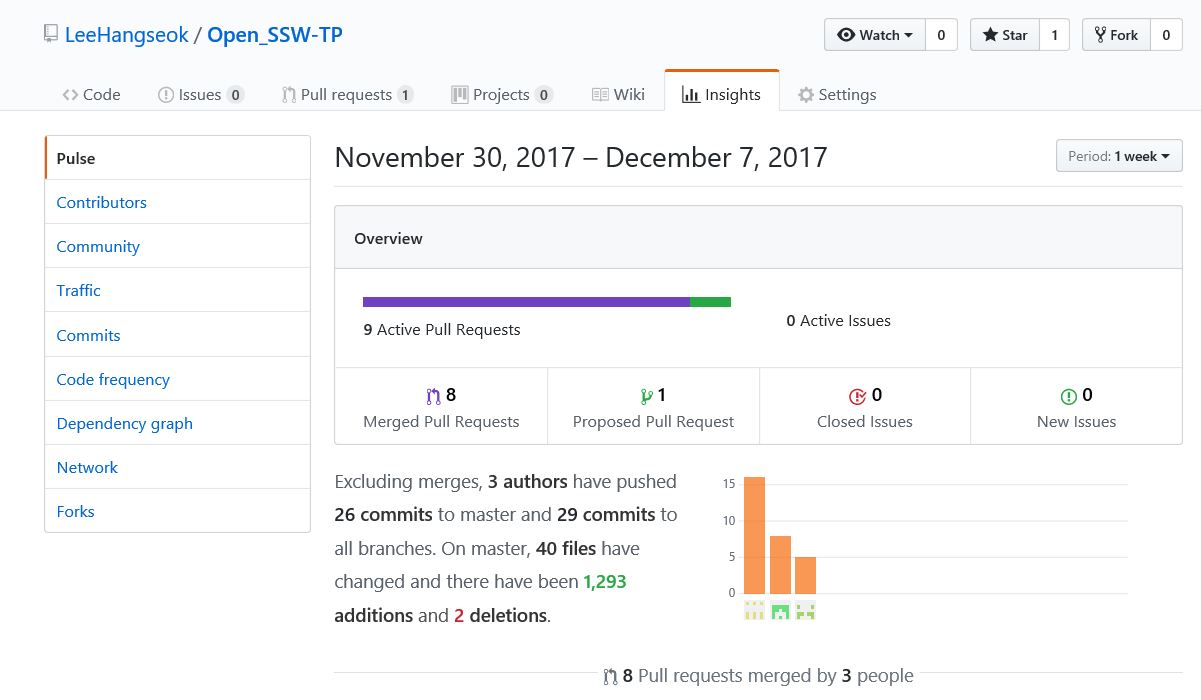
\includegraphics[scale=0.6]
{Image/Pulse.JPG}
\caption{Pulse 화면}
\label{fig:detect}
\end{figure}

 \section{Commit}
   \begin{figure}[h!]
\centering
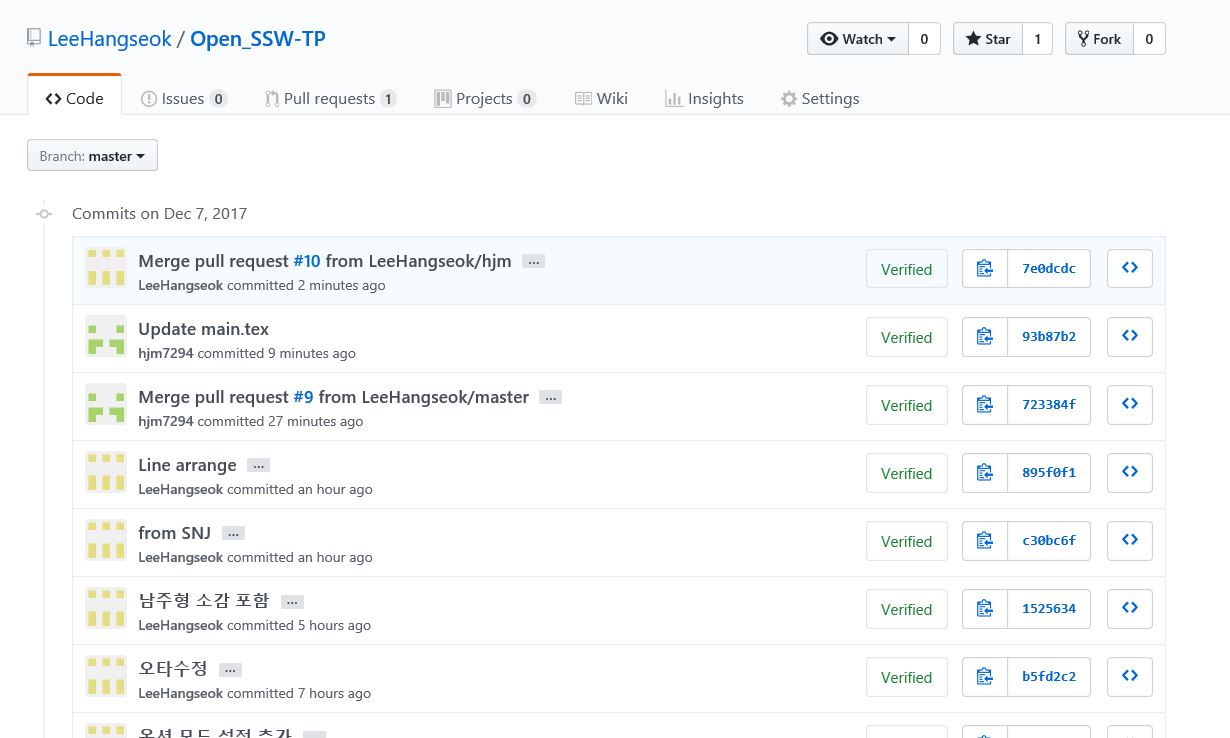
\includegraphics[scale=0.6]
{Image/Commit1.JPG}
\label{fig:detect}
\end{figure}


  \begin{figure}[h!]
\centering
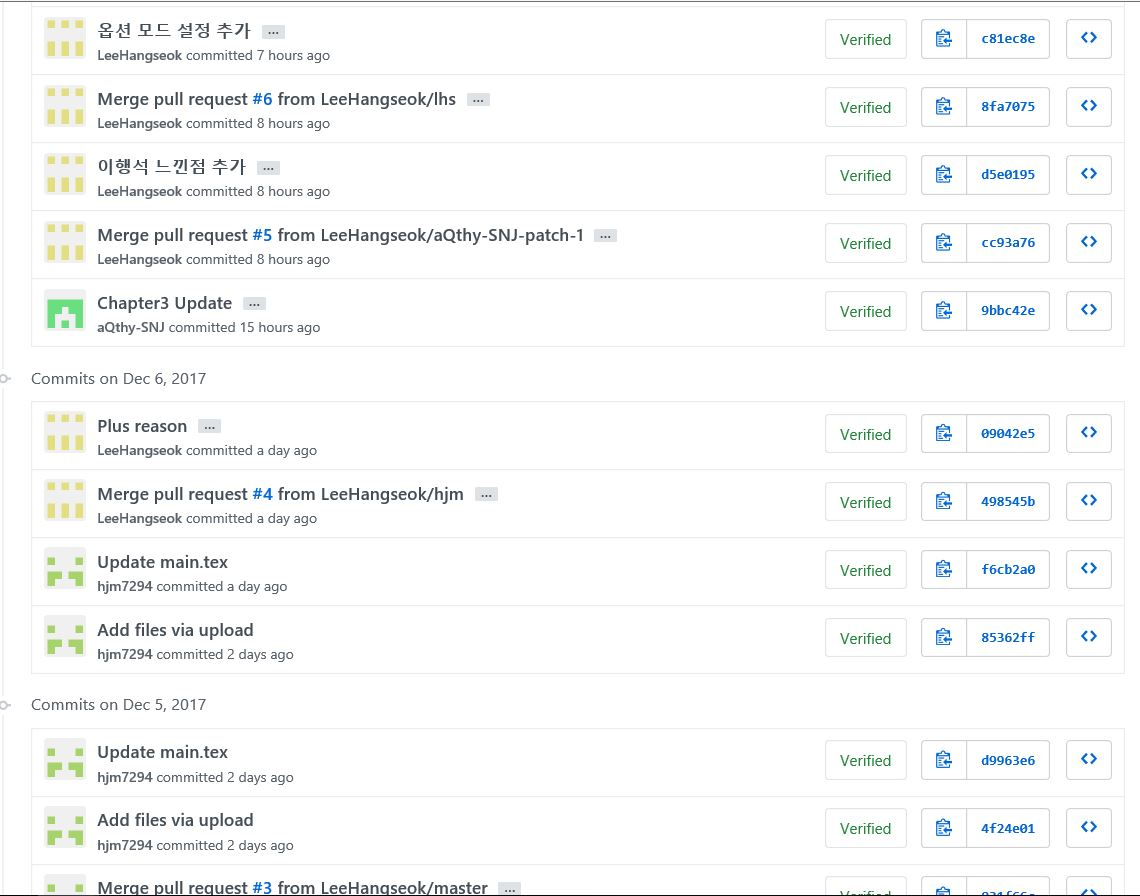
\includegraphics[scale=0.6]
{Image/Commit2.JPG}
\label{fig:detect}
\end{figure}

  \begin{figure}[h!]
\centering
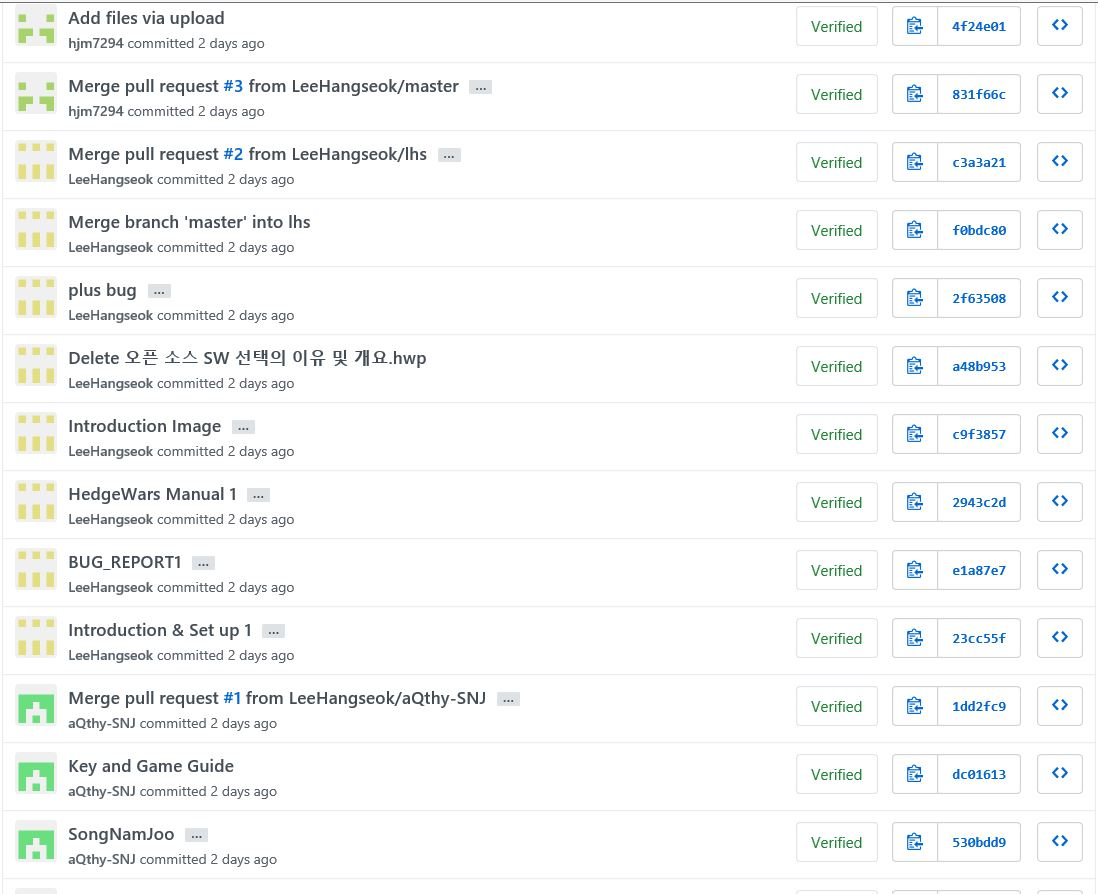
\includegraphics[scale=0.6]
{Image/Commit3.JPG}
\label{fig:detect}
\end{figure}

 \begin{figure}[h!]
\centering
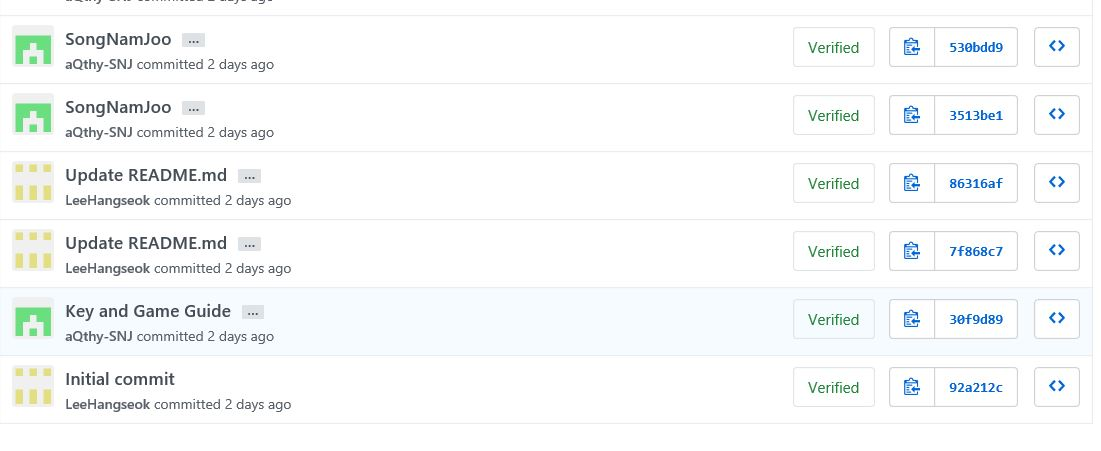
\includegraphics[scale=0.6]
{Image/Commit4.JPG}
\caption{Commit 내역 캡쳐본}
\label{fig:detect}
\end{figure}

\chapter{각 팀원별 역할 분담 및 느낀점}
 \\이행석 : 1장 오픈 소스 SW 개요 및 설치 
    \begin{itemize}
        \item 무료로 소스를 공개하는 점이 가장 인상깊었으며 특히 버그가 발생하더라도 많은 사용자들이 발견 하면 바로바로 리포트가 올라오거나 수정되는 모습이 자랑인 것 같습니다. 앞으로도 다양한 오픈 소스들을 활용하여 각 라이센스에 맞도록 활용 해야겠습니다.
        \item github의 경우 서로 다른 장소에 있더라도 각 팀원들이 branch에 commit 후 pull request를 보내 master 브랜치의 사용자가 승인만 하면 바로 merge 되는 점이 인상 깊었습니다.
    \end{itemize} 
    
    \\하지민 : 2장 게임 메뉴 및 옵션
    \begin{itemize}
        \item 조장이 궁금한것을 친절히 알려줘 쉽게 접근하여 차근차근 할 수 있었습니다.
        \item 처음에는 github를 사용하는것에 익숙하지 못해서 처음에는 힘들었지만 하면서 하면서 점점 익숙해지고나니 조원들과 파일을 보냈다 받아서 수정하고 다시보내는 작업보다 훨씬 간편하고 좋다는 생각을 하게되었습니다.
    \end{itemize}
    
    \\송남주 : 3장 키 설명 및 게임 방법
    \begin{itemize}
        \item 조원들과 의사 소통이 원활해서, 프로젝트가 매끄럽게 잘 진행되었습니다. 특히 조장이 직접 주도하여, 팀원들을 잘 이끌어주었습니다.
        \item 오픈 소스 소프트웨어라는 문구를 처음 들었을 때 공개적인 프로그램이기 때문에 마치 타 소프트웨어의 'Demo' 버전 처럼 완성도가 떨어지고, 제약이 많을 것이라고 생각했습니다. 하지만 이 Hedgewars라는 오픈 소스 소프트웨어를 해보면서, 이러한 편견이 사라졌습니다. 완성도도 높고, 과거 유행했던 게임 웜즈와 유사해서 옛 추억을 되새기기에도 좋았습니다. 
        \item 오픈소스SW보다 어려웠던 것은 Latex 사용과 Github였습니다. 중간고사 전에 배운 명령어와 Github는 과거 몇번 사용한 경험을 토대로 금방 활용할 수 있었지만, Latex은 처음 사용해보는 거라 당황스러웠습니다. 하지만 팀원들과 직접 Latex 각종 예시를 찾아보고 응용해보면서 금방 익숙해질 수 있었습니다.
    \end{itemize}

 \chapter{참고사이트 및 라이센스}
 \section{참고사이트}
 \begin{itemize}
     \item www.hedgewars.org(hedgewars 공식 홈페이지)
     \item www.https://ko.wikipedia.org/wiki/%ED%97%B7%EC%A7%80%EC%9B%8C%EC%A6%88(위키백과)
     \item https://namu.wiki/w/%ED%97%B7%EC%A7%80%EC%9B%8C%EC%A6%88?from=Hedgewars(나무위키)
 \end{itemize}
 \section{라이센스}
 \begin{itemize}
     \item GPL License
 \end{itemize}
\end{flushleft}
\end{document}
